\externaldocument{../3/chapter_modeling}
\externaldocument{../4/chapter_algorithm}
\startchapter{Feature Prototype On Atlantis}
\label{chapter:newsol}
In this section, I describe the design of the feature prototype of communication identification from the dual\_trace. This feature is implemented on Atlantis and is built on top of Atlantis' other features, such as ``memory reconstruction", ``function inspect" and ``views synchronization". Atlantis is an assembly trace analysis environment. It provides many powerful and novel features to assist assembly level execution trace analysis.\cite{huang2017atlantis} This prototype implemented the algorithms described in Chapter\ref{chapter:alo} as well as the user interfaces for the feature.

This prototype consist of four main components: 1) user defined setting for defining the concerned communication methods' function set. 2) a view that can parallelly present both traces in the dual\_trace. 3) two identification features: Stream identification and communication identification. 4) functionality that allow user to access the identification result.


\section{User Defined Function Set}\label{functionset}
As emphasized in Section\ref{windows}, the function set for each communication method can be different depends on the implementation solution of the method. Furthermore, there are so many communication methods in the real world and not all of them are being analyzed by the user. Instead of using hard coded function sets, a configuration file in Json format is used for the users to define their concerned communication methods and the corresponding function set. This function sets will be the input for the communication identification. All concerned communication methods have its own function set. The identification features implemented in this prototype iterate all methods in the Json configuration file named ``communicationMethods.json" and identify all communications of each method. This configuration includes the communication method, their function set for the communication events and the essential parameters of each function. A default template is given for user reference, this default template is generated by Atlantis when it was launched and stored in the .tmp folder in the trace analysis project folder. The default template example can be find in Section\ref{funcset}.

\subsection{Communication Methods' Implementation in Windows}\label{windows}
The implementation of the communication methods impact the algorithms to detect them. Hence, before discussing the algorithms, I provide the investigation result of the characteristics and the implementation of the communication methods in Windows. The goal of this investigation is to 1) obtain the system function set $fset$ for the concerned events in the communication and summarize the necessary parameters for further communication identification. and 2) understand the channel opening mechanism in order to identify the streams from the $etr$ and match the streams from two traces.

The implementations of four communication methods in Windows system are investigated. I reviewed the Windows APIs of the communication methods and their example code. For each communication method, a system function list is provided for reference. These lists contain function names, essential parameters. These functions are supported in most Windows operating systems, such as Windows 8, Window 7. The channel opening mechanisms of each method are described in detail and represented in diagrams.

Windows API set is very sophisticated and multiple solutions are provided to fulfil a communication method. It is impossible to enumerate all solutions for each communication method. I only give the most basic usage provided in Windows documentation. Therefore, the provided system function lists for the events should not be considered as the only combination or solution for each communication method. With the understanding of the model, it should be fairly easy to draw out lists for other solutions or other communication methods. 

Moreover, the instances of this model only demonstrate Windows C++ APIs. This model may be generalizable to other operating systems with the effort of understanding the APIs of those operating systems.

\subsubsection{Windows Calling Convention}
The Windows calling convention is important to know in this research. The communication identification relies not only on the system function names but also the key parameter values. In the assembly level execution traces, the parameter values is captured in the memory changes of the instructions. The memory changes are recognized by the register names or the memory address. The calling convention helps us to understand where the parameters are stored so that we can find them in the memory change map in the trace. Calling Convention is different for operating systems and the programming language. The Microsoft* x64 example calling convention is listed in \ref{convention} since we used dual-trace from Microsoft* x64 for case study in this work.

\subsubsection{Named Pipes}
In Windows, a named pipe is a communication method for the pipe server and one or more pipe clients. The pipe has a name, can be one-way or duplex. Both the server and clients can read or write into the pipe.\cite{WinNamedpipe} In this work, I only consider one server versus one client communication. One server to multiple clients scenario can always be divided into multiple server and client communications thanks to the characteristic that each client and server communication has a separate conduit. The server and client are endpoints in the communication. We call the server ``server endpoint" while the client ``client endpoint".  The server endpoint and client endpoint of a named pipe share the same pipe name, but each endpoint has its own buffers and handles. 

There are two modes for data transfer in the named pipe communication method, synchronous and asynchronous.  Modes affect the functions used to complete the send and receive operation. I list the related functions for both synchronous mode and asynchronous mode. The create channel functions for both modes are the same but with different input parameter value. The functions for send and receive message are also the same for both cases. However, the operation of the send and receive functions are different for different modes. In addition, an extra function \textit{GetOverlappedResult} is being called to check if the sending or receiving operation finish, the output message will be stored in the overlap structure whose memory address saved in the function's output parameter Overlap Structure Address. Table\ref{synfunctions} lists the functions of the events for synchronous mode while Table\ref{asynfunctions} lists the functions of the events for the asynchronous mode for a Named pipe communication.

    \begin{table}[H]
        \centering
        \small
        \caption{Function List  of events for Synchronous Named Pipe}
        \label{synfunctions}
        \begin{tabular}{|l|l|l|l|l|}
            \hline
             \multirow{2}{*}{\textbf{Event}} &
               \multicolumn{2}{c|}{\textbf{Server Endpoint}} &
               \multicolumn{2}{c|}{\textbf{Client Endpoint}} \\
             \cline{2-5}
              & \textbf{Function}& \textbf{Parameters} & \textbf{Function} & \textbf{Parameters}  \\
             \hline
             \multirow{2}{*}{{\textbf{Channel Open}}}
             &\multirow{2}{*}{{CreateNamedPipe}} &  RAX: File Handler & \multirow{2}{*}{CreateFile} &  RAX: File Handler\\
              \cline{3-3} \cline{5-5}
             &&  RCX: File Name &  &  RCX: File Name\\
            \hline
             {{\textbf{Channel Open}}}
             &{ConnectNamedPipe} & {RCX: File Handler} & & \\
            \hline
             \multirow{3}{*}{{\textbf{Send}}}
             &\multirow{3}{*}{WriteFile} &  RCX: File Handle & \multirow{3}{*}{WriteFile} &  RCX: File Handle\\
              \cline{3-3} \cline{5-5}
             &&  RDX: Buffer Address &  &  RDX: Buffer Address\\
                           \cline{3-3} \cline{5-5}
             & &  R9: Message Length &  &  R9: Message Length\\
            \hline
             \multirow{3}{*}{{\textbf{Receive}}}
             & \multirow{3}{*}{ReadFile}&  RCX: File Handle & \multirow{3}{*}{ReadFile} &  RCX: File Handle\\
              \cline{3-3} \cline{5-5}
              &&  RDX: Buffer Address &  &  RDX: Buffer Address\\
                           \cline{3-3} \cline{5-5}
             & &  R9: Message Length &  &  R9: Message Length\\
            \hline
           {{\textbf{Channel Close}}}
             &{CloseHandle} & {RCX: File Handler} & {CloseHandle} & {RCX: File Handler}\\
            \hline
             {{\textbf{Channel Close}}}
             &{DisconnectNamedPipe} & {RCX: File Handler} & {DisconnectNamedPipe} & {RCX: File Handler}\\
            \hline
        \end{tabular}
    \end{table}

    \begin{table}[H]
        \centering
        \small
        \caption{Function List  of events for Asynchronous Named Pipe}
        \label{asynfunctions}
        \begin{tabular}{|l|l|l|l|l|}
            \hline
             \multirow{2}{*}{\textbf{Event}} &
               \multicolumn{2}{c|}{\textbf{Server Endpoint}} &
               \multicolumn{2}{c|}{\textbf{Client Endpoint}} \\
             \cline{2-5}
              & \textbf{Function}& \textbf{Parameters} & \textbf{Function} & \textbf{Parameters}  \\
             \hline
             \multirow{2}{*}{{\textbf{Channel Open}}}
             &\multirow{2}{*}{{CreateNamedPipe}} &  RAX: File Handler & \multirow{2}{*}{CreateFile} &  RAX: File Handle\\
              \cline{3-3} \cline{5-5}
             &&  RCX: File Name &  &  RCX: File Name\\
            \hline
            {{\textbf{Channel Open}}}
             &{ConnectNamedPipe} & {RCX: File Handler} & & \\
            \hline
             \multirow{3}{*}{{\textbf{Send}}}
             &\multirow{3}{*}{WriteFile} &  RCX: File Handle & \multirow{3}{*}{WriteFile} &  RCX: File Handle\\
              \cline{3-3} \cline{5-5}
             &&  RDX: Buffer Address &  &  RDX: Buffer Address\\
                           \cline{3-3} \cline{5-5}
             & &  R9: Message Length &  &  R9: Message Length\\
            \hline
            \multirow{3}{*}{{\textbf{Receive}}}
             & \multirow{3}{*}{ReadFile}&  RAX: File Handle & \multirow{3}{*}{ReadFile} &  RCX: File Handle\\
              \cline{3-3} \cline{5-5}
              &&  RDX: Buffer Address &  &  RDX: Buffer Address\\
                           \cline{3-3} \cline{5-5}
             & &  R9: Message Length &  &  R9: Message Length\\
              \hline
               \multirow{2}{*}{{\textbf{Receive}}}
             & \multirow{2}{*}{GetOverlapped-}&  RCX: File Handler & \multirow{2}{*}{GetOverlapped-} &  RCX: File Handler\\
              \cline{3-3} \cline{5-5}
             &  \multirow{2}{*}{Result} &  RDX:  Overlap  &  \multirow{2}{*}{Result }&  RDX:  Overlap \\
              &  &  Structure address &  &  Structure Address\\
            \hline                       
            \textbf{Channel Close}
             &{CloseHandle} &{RCX: File Handler} & {CloseHandle} &  {RCX: File Handler}\\
            \hline
           {{\textbf{Channel Close}}}
             &{DisconnectNamedPipe} & {RCX: File Handler} & {DisconnectNamedPipe} & {RCX: File Handler}\\
            \hline
        \end{tabular}
    \end{table}



\subsubsection{Message Queue}
Similar to Named Pipe, Message Queue's implementation in Windows also has two modes, synchronous and asynchronous. Moreover, the asynchronous mode further divides into two operations, one with callback function while the other without. With the callback function, the callback function would be called when the send or receive operations finish. Without callback function, the general function \textit{MQGetOverlappedResult} should be called by the endpoints to check if the message sending or receiving operation finish, the output message will be stored in the overlap structure whose memory address saved in the function's output parameter Overlap Structure Address. Table\ref{msmqsynfunctions} lists the functions for synchronous mode while Table\ref{msmqasynfunctionscallback} and Table\ref{msmqasynfunctions} list the functions for the asynchronous mode with and without callback. 

    \begin{table}[H]
        \centering
        \caption{Function List  of events for Synchronous MSMQ}
        \label{msmqsynfunctions}
        \begin{tabular}{|l|l|l|}
            \hline
             \textbf{Event} & \textbf{Function}& \textbf{Parameters}  \\
             \hline
             \multirow{2}{*}{{\textbf{Channel Open}}}
             &\multirow{2}{*}{{MQOpenQueue}} &  RAX: Queue Handler\\
              \cline{3-3} 
             & &  RCX: Queue Format Name\\
            \hline
             \multirow{2}{*}{{\textbf{Send}}}
             &\multirow{2}{*}{MQSendMessage} &  RCX: Queue Handle \\
              \cline{3-3} 
             &&  RDX: Message description structure Address \\
            \hline
             \multirow{2}{*}{{\textbf{Receive}}}
             & \multirow{2}{*}{MQReceiveMessage}&  RCX: Queue Handle \\
              \cline{3-3} 
              &&  R9: Message description structure Address \\
            \hline
            \textbf{Channel Close} &MQCloseQueue & RCX: Queue Handler \\
            \hline
        \end{tabular}
    \end{table}


    \begin{table}[H]
        \centering
        \caption{Function List of events for Asynchronous MSMQ with Callback}
        \label{msmqasynfunctionscallback}
        \begin{tabular}{|l|l|l|}
            \hline
             \textbf{Event} & \textbf{Function}& \textbf{Parameters}  \\
             \hline
             \multirow{2}{*}{{\textbf{Channel Open}}}
             &\multirow{2}{*}{{MQOpenQueue}} &  RAX: Queue Handler\\
              \cline{3-3} 
             & &  RCX: Queue Format Name\\
            \hline
             \multirow{2}{*}{\textbf{Send}}
             &\multirow{2}{*}{MQSendMessage} &  RCX: Queue Handle \\
              \cline{3-3} 
             &&  RDX: Message description structure Address \\
            \hline
             \multirow{2}{*}{\textbf{Receive}}
             & \multirow{2}{*}{MQReceiveMessage}&  RCX: Queue Handle \\
              \cline{3-3} 
              &&  R9: Message description structure Address \\
             \hline
             \textbf{Receive}
              &CallbackFuncName&  Parameters for the callback function. \\
            \hline
            \textbf{Channel Close} &MQCloseQueue & RCX: Queue Handler \\
            \hline
        \end{tabular}
    \end{table}

    \begin{table}[H]
        \centering
        \caption{Function List  of events for Asynchronous MSMQ without Callback}
        \label{msmqasynfunctions}
        \begin{tabular}{|l|l|l|}
            \hline
             \textbf{Event} & \textbf{Function}& \textbf{Parameters}  \\
             \hline
             \multirow{2}{*}{{\textbf{Channel Open}}}
             &\multirow{2}{*}{{MQOpenQueue}} &  RAX: Queue Handler\\
              \cline{3-3} 
             & &  RCX: Queue Format Name\\
            \hline
             \multirow{2}{*}{{\textbf{Send}}}
             &\multirow{2}{*}{MQSendMessage} &  RCX: Queue Handle \\
              \cline{3-3} 
             &&  RDX: Message description structure Address \\
            \hline
             \multirow{2}{*}{{\textbf{Receive}}}
             & \multirow{2}{*}{MQReceiveMessage}&  RCX: Queue Handle \\
              \cline{3-3} 
              &&  R9: Message description structure Address \\
              \hline
              \textbf{Receive} 
              & MQGetOverlappedResult &  RCX: Overlap Structure address  \\
            \hline
            \textbf{Channel Close} &MQCloseQueue & RCX: Queue Handler \\
            \hline
        \end{tabular}
    \end{table}
    

    
\subsubsection{TCP and UDP}
In Windows programming, these two methods shared the same set of APIs regardless the input parameter values and operation behaviour are different. In Windows socket solution, one of the two endpoints is the server while the other one is the client. Table \ref{tcpupdfunctions} lists the functions of a UDP or TCP communication. 
  \begin{table}[H]
        \centering
        \caption{Function List  of events for TCP and UDP}
        \label{tcpupdfunctions}
        \begin{tabular}{|l|l|l|l|l|}
            \hline
             \multirow{2}{*}{\textbf{Event}} &
               \multicolumn{2}{c|}{\textbf{Server Endpoint}} &
               \multicolumn{2}{c|}{\textbf{Client Endpoint}} \\
             \cline{2-5}
              & \textbf{Function}& \textbf{Parameters} & \textbf{Function} & \textbf{Parameters}  \\
             \hline
             \textbf{Channel Open}
             &socket&  RAX: Socket Handle & socket &  RAX: Socket Handle\\
             \hline
                \multirow{2}{*}{{\textbf{Channel Open}}}
              &\multirow{2}{*}{{bind}} &  RCX: Socket Handle & \multirow{2}{*}{connect} &  RCX: Socket Handle\\
              \cline{3-3} \cline{5-5}
             &&  RDX: Server Address $\&$ Port &  &  RDX: Server Address $\&$ Port\\
            \hline
                \multirow{3}{*}{{\textbf{Channel Open}}}
             &\multirow{3}{*}{{accept}} &  RAX: New Socket Handle && \\
              \cline{3-3} 
             &&  RCX:  Socket Handle &  & \\
             \cline{3-3} 
             &&  RDX: Client Address $\&$ Port &  &  \\
            \hline
             \multirow{2}{*}{{\textbf{Send}}}
             &\multirow{2}{*}{send} &  RCX: New Socket Handle & \multirow{2}{*}{send} &  RCX: Socket Handle\\
              \cline{3-3} \cline{5-5}
             &&  RDX: Buffer Address &  &  RDX: Buffer Address\\
           \hline
              \multirow{2}{*}{{\textbf{Receive}}}
             & \multirow{2}{*}{recv}&  RCX: New Socket Handle & \multirow{2}{*}{recv} &  RCX: Socket Handle\\
              \cline{3-3} \cline{5-5}
              &&  RDX: Buffer Address &  &  RDX: Buffer Address\\
            \hline
          {{\textbf{Channel Close}}}&
            {closesocket} & {RCX: New Socket Handle} &{closesocket} & {RCX: Socket Handle}\\
            \hline
        \end{tabular}
    \end{table} 
   

\section{Parallel Editor View For Dual\_Trace}
The dual\_trace consist of two execution traces which are interacting with each other. Presenting them in the same view makes the analysis for the user much easier. The strategy to open parallel editor view is that open one trace as the normal one and the other as the dual\_trace of the current opened one. A new menu option in the project navigation view are created to open the second trace as the dual\_trace of the current active trace. The implementation of the parallel editor take the advantage of the existing SWT of Eclipse plug-in development. The detail of the implementation can be found in Section\ref{paralleleditor}. Figure\ref{opendualtracemenu} shows this menu option and Figure\ref{paralleleditor} shows the parallel editor view.

\begin{figure}[H]
\centerline{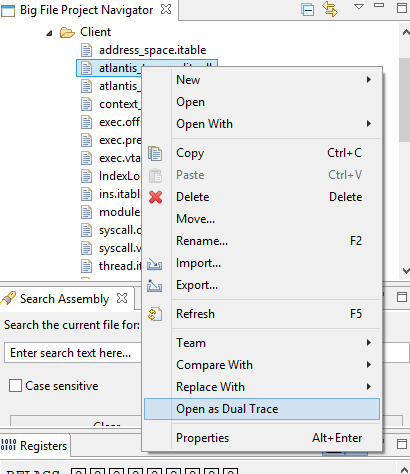
\includegraphics[scale=0.7]{Figures/opendualtracemenu}}
 \caption{Menu Item for opening Dual\_trace}
\label{opendualtracemenu}
\end{figure}

\begin{figure}[H]
\centerline{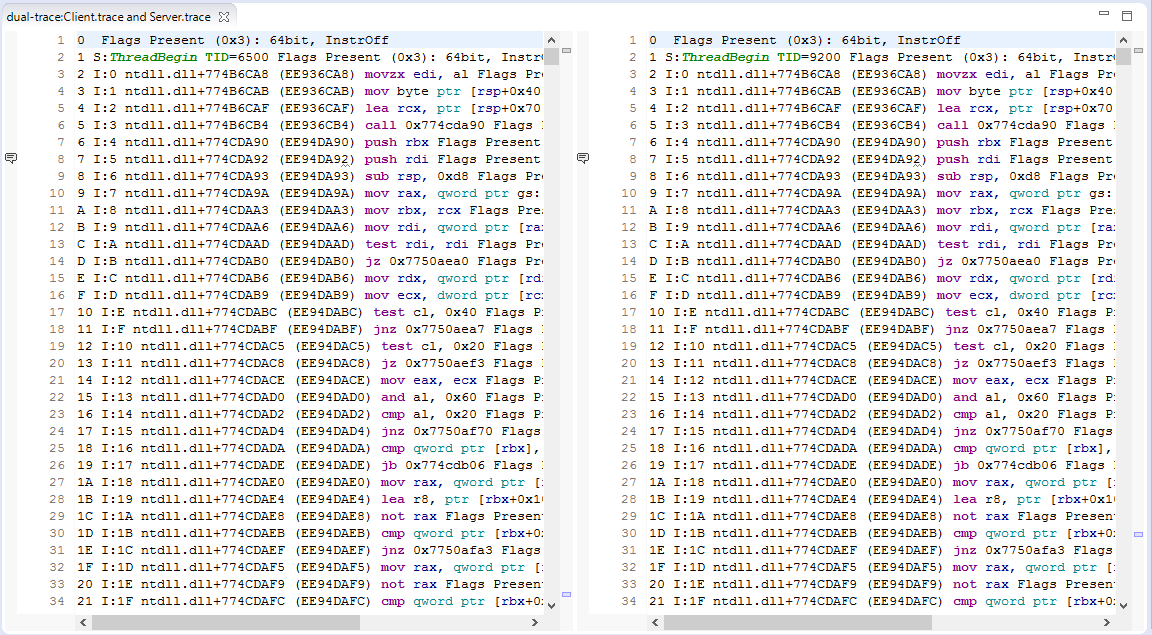
\includegraphics[scale=0.6]{Figures/paralleleditor}}
 \caption{Parallel Editor View}
\label{paralleleditor}
\end{figure}



\section{Identification Features}
I implemented two identification features, one is stream identification for both traces in the dual\_trace, the other is the communication identification. These two features align to the ``stream identification algorithm" and ``communication identification algorithm" designed in Chapter\ref{chapter:alo}. The implementation of these two identification features relies on the existing ``function inspect" feature of Atlantis. The called functions' name can be inspected  by  search of the symbolic name in the executable binary or any DLLs which used by the program at the time when it is traced. By importing the DLLs and executable binary, Atlantis can recognize the function call from the execution trace by the function names. Therefore the corresponding Dlls or executable binaries for both traces in the dual\_trace have to be loaded into Atlantis before conducting the identification.

A new menu ``Dual\_trace Tool" with three menu options is designed for these two identification features. In this menu, two options are for conducting the identification which are ``Stream Identification" and ``Communication Identification" while one is for loading the DLLs and executable binary which is ``Load Library Exports". Currently, the ``Load library export" function can only load libraries for the trace in the active editor. So this item in the menu has to be run twice separately for each trace of the dual\_trace.  Figure\ref{dualtracetoolmenu} shows this new menu in Atlantis. When the user perform any of the identification features, there is the prompt dialog as shown in Figure\ref{methods} which asks the user what communication methods they want to identify from the dual\_trace. This list is provided by the configuration file I mention in Section\ref{functionset}. The user can select one or multiple methods. 

\begin{figure}[H]
\centerline{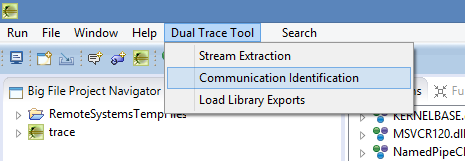
\includegraphics{Figures/dualtracetoolmenu}}
 \caption{Dual\_trace Tool Menu}
\label{dualtracetoolmenu}
\end{figure}

\begin{figure}[H]
\centerline{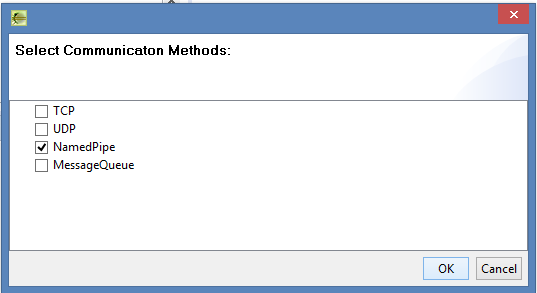
\includegraphics[scale=0.8]{Figures/methods}}
 \caption{Prompt Dialog for Communication Selection}
\label{methods}
\end{figure}

A new view named ``Communication" is designed for presenting the result of the identification of streams and communications. Since the user can have multiple selection for communication methods they concern, the output identification result contains all the identified communications or streams of all the concerned communication methods and the identified results are clustered by methods. There are two sub tables in this view, the left one is for the stream identification result while the left one is for communication identification result. The reason for putting this two result in the same view is for easy access and comparison of the data for the users. Figure\ref{idenview} shows this view with result data in it. Each time when the user rerun the identification features the result in the corresponding table will be refreshed to show only the latest identification result. But the other table will not be affected. For example, if the user run the ``Stream Identification" feature first, the stream identification result will show on the left table of the view. And then the user run the ``communication Identification", the communication identification result will be shown on the right table while the left one still holding the last stream identification result.

\begin{figure}[H]
\centerline{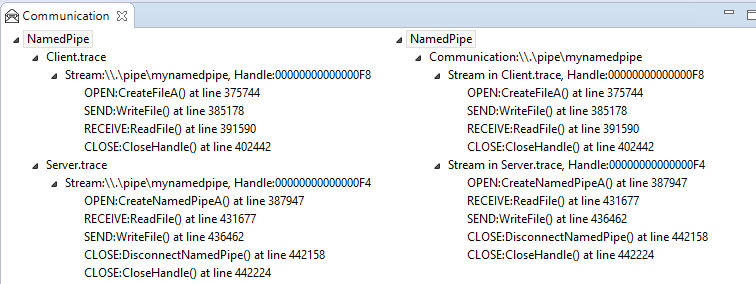
\includegraphics[scale=0.7]{Figures/idenview}}
 \caption{Communication View for Showing Identification Result}
\label{idenview}
\end{figure}

\section{Identification Result View and Result Navigation}
Atlantis is a analysis environment that has various views to allow user access to different information from the trace, such as the memory and register state of the current instruction line. Moreover, these views synchronize automatically with the editor view. These functionality and information also benefit the communication analysis of the dual\_trace. Providing the user a way to navigate from the identified result to the traces in the editors allows them to take advantage of the current existing functionality of Atlantis and make their analysis of the dual\_trace more efficient.

In the result list, each event entry is corresponding to a function call. The functions were called at function call line and all the inputs of the function calls can be recovered from the memory state of this instruction line. The functions returned at the return instruction lines, all the outputs of the function calls can be recovered in the memory state of the the return instruction line. From the event entries, this implementation provide two different ways for the user to navigate back to where the function begins and ends. When the user ``double click" on an entry, it will bring the user to the start line of the function in the corresponding trace editor. When the the right click on the event entry, a prompted menu with the option ``Go To Line of Function End" will show up as in Figure\ref{gotoend}. Clicking on this option will bring the user to the return line of this function in the trace editor. All other views update immediately with this navigation. 

\begin{figure}[H]
\centerline{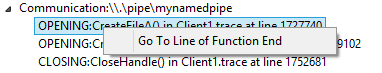
\includegraphics{Figures/gotoend}}
 \caption{Right Click Menu on Event Entry}
\label{idenview}
\end{figure}

Moreover, the ``remove" option as shown in Figure\ref{remove} in the right click menu on the ``stream“ or ``communication" entries is provided for the user to remove the selected ``stream" or ``communication" entry. This provides the user the flexibility to get rid of the data that they don't care.

\begin{figure}[H]
\centerline{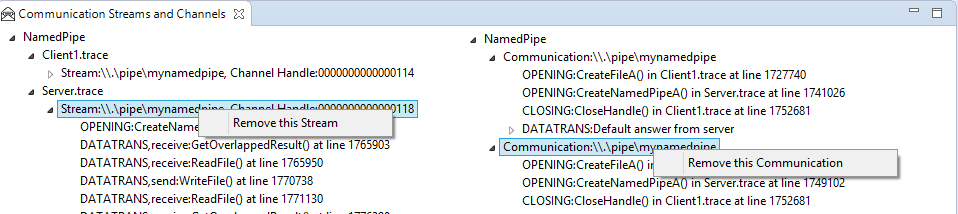
\includegraphics[scale=0.7]{Figures/remove}}
 \caption{Right Click Menu on Event Entry}
\label{remove}
\end{figure}

\section{Data Structures for Identified Communications}
The information of identified communications should be organized properly for the user. In this section, I define the output data structures to fulfil this requirement. There are totally two major data set. The first one is clustered as communications aligning the definition at Section\ref{definition}. The second one is clustered by endpoints in the traces. The reason to provide the second data set is due to the false negative errors of the channel identification. The identified endpoint lists of the traces provide more original data information. So with other assistant information and the access of this relatively original information of the dual-trace, the user has more flexibility to analysis the dual-trace. The data structures have been used in the algorithms implicitly.

\begin{algorithm}[H]
\DontPrintSemicolon
\caption{{\bf Data Structure for Identified Communications} \label{communicationlData}}
$cs \leftarrow Map \langle String, List \langle Communication \rangle \rangle$;\tcp*[f]{the key is the communication method}\;  
$str \leftarrow Map \langle String, List \langle Stream \rangle \rangle$;  \tcp*[f]{the key is the communication method}\;  
\Struct{Communication}{
  Stream s0 \tcp*[f]{s0 is from $tr0$ of the dual-trace}\;  
  Stream s1 \tcp*[f]{s1 is from $tr1$ of the dual-trace}\;  
  DataMatch dataMatch\;  
}


\Union{DataMatch}{
  DataUnionMatch \quad  unionMatch \tcp*[f]{For data union verification}\;  
  List $\langle$ EventMatch $\rangle$ \enspace eventMatchs \tcp*[f]{For data event verification}\;  
}

\Struct{DataUnionMatch}{
  String sData1 \tcp*[f]{send data union of endpoint1}\;  
  String rData1 \tcp*[f]{receive data union of endpoint1,substring of sData2}\;  
  String sData2 \tcp*[f]{send data union of endpoint2}\;  
  String rData2 \tcp*[f]{receive data union of endpoint2,substring of sData1}\; 
}

\Struct{EventMatch}{
  Event \quad \quad event1 \tcp*[f]{event1 is from enpoint1}\;  
  Event \quad \quad event2 \tcp*[f]{event2 is from enpoint2}\;  
}


\Struct{Stream}{
  Int \quad \quad handle\;
  List $\langle$ Event $\rangle$ \enspace openStream\;
  List $\langle$ Event $\rangle$ \enspace closeStream\;
  List $\langle$ Event $\rangle$ \enspace sendStream\;
  List $\langle$ Event $\rangle$ \enspace receiveStream\; 
}

\Struct{Event}{
   Int \quad \quad \quad \quad \quad \quad \quad \quad stratline\;
   Int \quad \quad \quad \quad \quad \quad \quad \quad endline\;
   Map $\langle$ String, String $\rangle$ \enspace inputs\; 
   Map $\langle$ String, String $\rangle$ \enspace outputs\; 
}

\end{algorithm} 


